\documentclass[../main.tex]{subfiles}
\usepackage{graphicx}
\usepackage{subcaption}
\usepackage{adjustbox}

\begin{document}

\begin{enumerate}
    \item Fuente de chispero y chispero electrónico.
    \item Conexiones para el aire comprimido. 
    \item Tablero con superficie de vidrio.
    \item Papel electrónico A3 y papel bond tamaño A3.
    \item Disco de 10 cm de diámetro.
    \item Dos resortes y cinco pesas.
    \item Regla milimetrada.
    \item Una balanza.
    \item Un nivel de burbuja.
\end{enumerate}

\subsection*{Imágenes del equipo utilizado}

\begin{figure}[H]

    \begin{tabular}{c c}
        
    \begin{subfigure}{0.5\textwidth} 
        \centering
        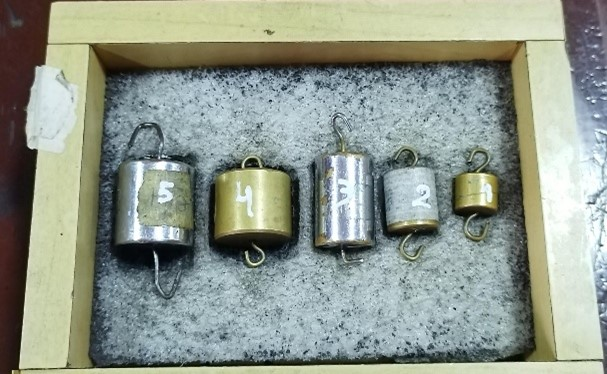
\includegraphics[width=0.8\linewidth, height=3.5cm]{images/materiales/mat1.jpg}
        \caption{Pesas}
        \label{fig:pesas}
    \end{subfigure}
    &
    \begin{subfigure}{0.5\textwidth}  
        \centering
        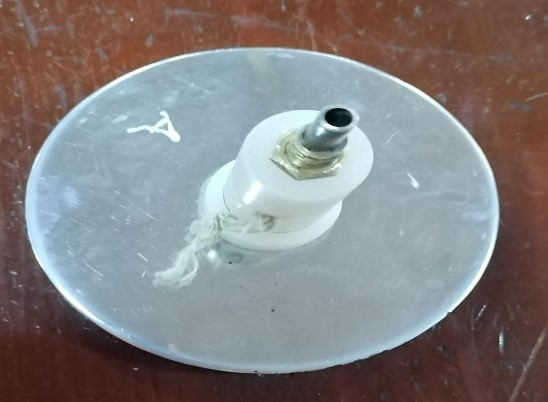
\includegraphics[width=0.8\linewidth, height=3.5cm]{images/materiales/mat2.jpg}
        \caption{Disco}
        \label{fig:disco}
    \end{subfigure} \\
    
    \begin{subfigure}{0.5\textwidth} 
        \centering
        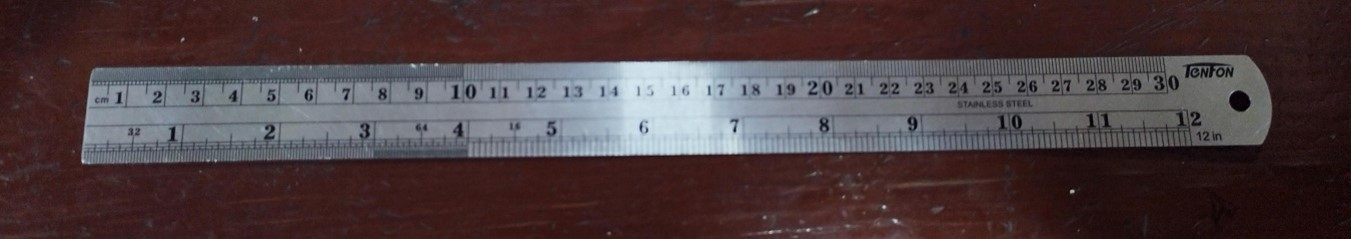
\includegraphics[width=0.8\linewidth, height=3.5cm]{images/materiales/mat3.jpg}
        \caption{Regla graduada}
        \label{fig:regla}
    \end{subfigure}
    &
    \begin{subfigure}{0.5\textwidth}
        \centering
        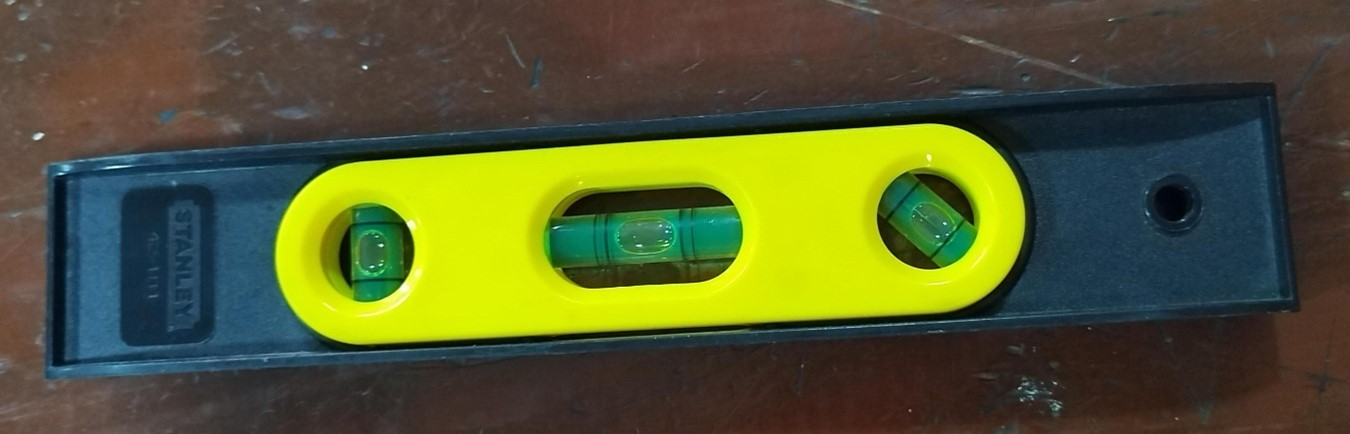
\includegraphics[width=0.8\linewidth, height=3.5cm]{images/materiales/mat4.jpg}
        \caption{Nivel}
        \label{fig:nivel}
    \end{subfigure} \\
    
    \begin{subfigure}{0.5\textwidth} 
        \centering
        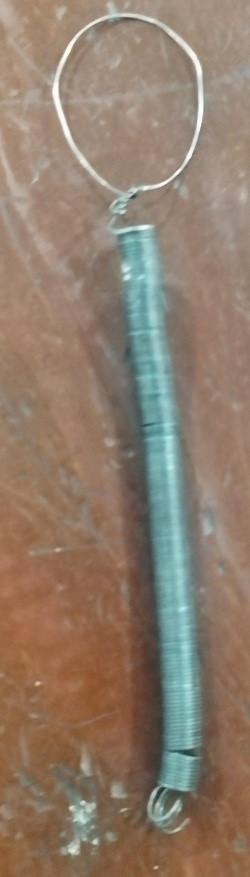
\includegraphics[height=0.8\linewidth,angle=90]{images/materiales/mat5.jpg}
        \caption{Resorte A}
        \label{fig:resortea}
    \end{subfigure}
    &
    \begin{subfigure}{0.5\textwidth}  
        \centering
        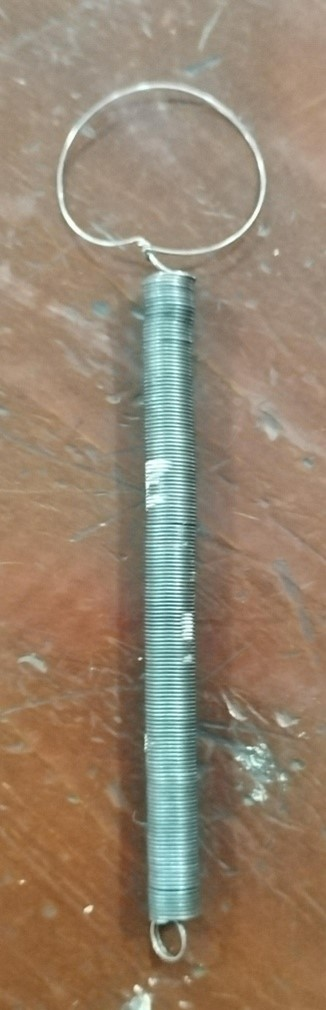
\includegraphics[height=0.8\linewidth,angle=90]{images/materiales/mat6.jpg}
        \caption{Resorte B}
        \label{fig:resorteb}
    \end{subfigure} \\
    
    \begin{subfigure}{0.5\textwidth}  
        \centering
        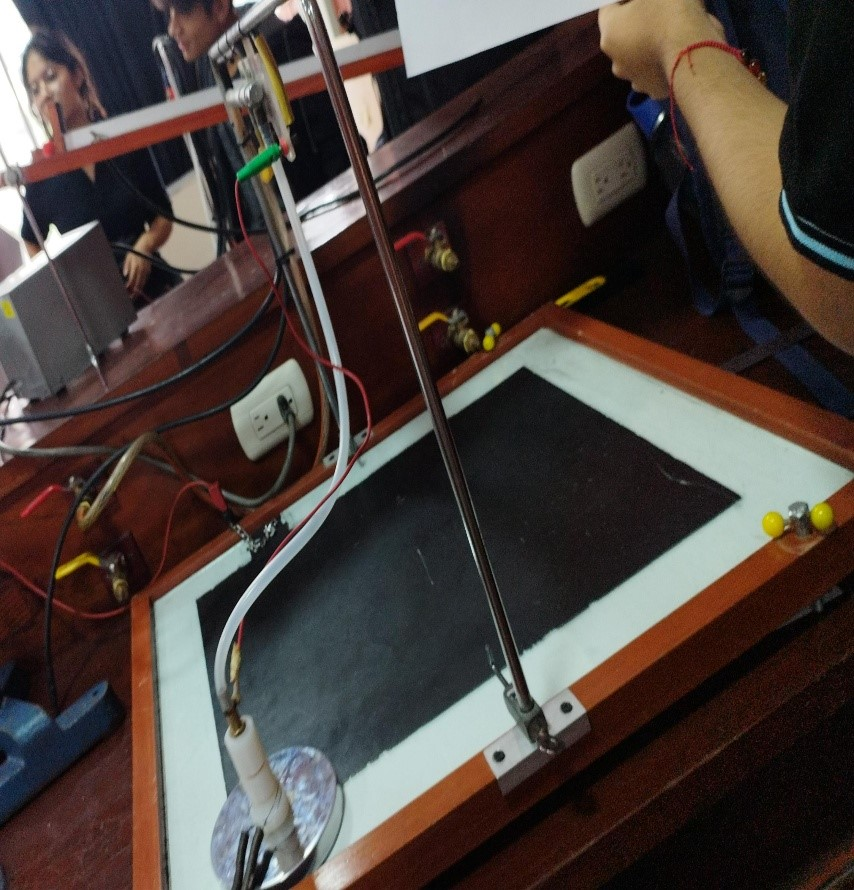
\includegraphics[width=0.8\linewidth, height=3.5cm]{images/materiales/mat7.jpg}
        \caption{Tablero}
        \label{fig:tablero}
    \end{subfigure} \\
    \end{tabular}
    
    \caption{Materiales utilizados.}
    \label{fig:materiales}
\end{figure}

\end{document}